\documentclass[11pt, english]{article}
\usepackage{graphicx}
\usepackage[colorlinks=true, linkcolor=blue]{hyperref}
\usepackage[english]{babel}
\selectlanguage{english}
\usepackage[utf8]{inputenc}
\usepackage[svgnames]{xcolor}
\usepackage{svg}

\usepackage{listings}
\usepackage{afterpage}
\pagestyle{plain}

\definecolor{dkgreen}{rgb}{0,0.6,0}
\definecolor{gray}{rgb}{0.5,0.5,0.5}
\definecolor{mauve}{rgb}{0.58,0,0.82}

%\lstset{language=R,
%    basicstyle=\small\ttfamily,
%   stringstyle=\color{DarkGreen},
%    otherkeywords={0,1,2,3,4,5,6,7,8,9},
%    morekeywords={TRUE,FALSE},
%    deletekeywords={data,frame,length,as,character},
%    keywordstyle=\color{blue},
%    commentstyle=\color{DarkGreen},
%}

\lstset{frame=tb,
language=R,
aboveskip=3mm,
belowskip=3mm,
showstringspaces=false,
columns=flexible,
numbers=none,
keywordstyle=\color{blue},
numberstyle=\tiny\color{gray},
commentstyle=\color{dkgreen},
stringstyle=\color{mauve},
breaklines=true,
breakatwhitespace=true,
tabsize=3
}

\usepackage{here}


\textheight=21cm
\textwidth=17cm
%\topmargin=-1cm
\oddsidemargin=0cm
\parindent=0mm
\pagestyle{plain}

%%%%%%%%%%%%%%%%%%%%%%%%%%
% La siguiente instrucción pone el curso automáticamente%
%%%%%%%%%%%%%%%%%%%%%%%%%%

\usepackage{color}
\usepackage{ragged2e}

\global\let\date\relax
\newcounter{unomenos}
\setcounter{unomenos}{\number\year}
\addtocounter{unomenos}{-1}
\stepcounter{unomenos}
\gdef\@date{ Course \arabic{unomenos}/ 2019}

\begin{document}

\begin{titlepage}

\begin{center}
\vspace*{-1in}
\begin{figure}[htb]
\begin{center}
\centering
\begin{tabular}{@{}cccc@{}}

\includegraphics[width=6cm]{images/EscudoUNAM.png}
\hspace*{1.2in}

\includegraphics[width=6cm]{images/logoIng.png}
\end{tabular}
\end{center}
\end{figure}

FACULTAD DE INGENIERÍA - \@date\\
\vspace*{0.15in}
SECRETARÍA/DIVISIÓN: DIVISIÓN DE INGENIERÍA ELÉCTRICA \\
ÁREA/DEPARTAMENTO: INGENIERÍA EN COMPUTACIÓN \\
\vspace*{0.4in}
\begin{large}
LABORATORIO DE COMPUTACIÓN GRÁFICA E INTERACCIÓN HUMANO COMPUTADORA:\\
\end{large}
\vspace*{0.2in}
\begin{Large}
\textbf{Proyecciones y puertos de vista. Transformaciones Geométricas } \\
\end{Large}
\vspace*{0.3in}
\vspace*{0.3in}
\begin{large}
Reynaldo Martell Avila \\
\end{large}
\vspace*{0.5in}
\vspace*{0.5in}
\begin{large}
\textbf{PRÁCTICA 3} \\
\end{large}
\end{center}
\end{titlepage}

\newcommand{\CC}{C\nolinebreak\hspace{-.05em}\raisebox{.4ex}{\tiny\bf +}\nolinebreak\hspace{-.10em}\raisebox{.4ex}{\tiny\bf +}}
\def\CC{{C\nolinebreak[4]\hspace{-.05em}\raisebox{.4ex}{\tiny\bf ++}}}

\tableofcontents

\newpage
\section{Objetivos de aprendizaje}
\subsection{Objetivos generales:}
El alumno repasará como crear buffers de OpenGL, leer archivos, comprenderá los
diferentes tipos de proyección y las funciones de la librería glm para crear éstas, así como
comprenderá los diferentes sistemas de referencia de OpenGL. Del mismo modo practicará
como colocar en la escena diferentes geometrías.
\subsection{Objetivos específicos:}
El alumno practicará crear geometrías con índices, revisará los sistemas de referencia que
se aplican en OpenGL, comprenderá la utilización de la matriz de modelo, vista, proyección
y la zona de dibujo.
\section{Recursos a emplear}
\subsection{Software}
Sistema Operativo: Windows 7
Ambiente de Desarrollo: Visual Studio 2017.
\subsection{Equipos}
Los equipos de cómputo con los que cuenta el laboratorio de Computación Gráfica
\subsection{Instrumentos}
\section{Fundamento Teórico}
\begin{itemize}
\item \textbf{Presentación de conceptos.} \\
Se mostrará la utilización de índices, se revisará como crear los shaders de fragmento y
vértices desde un archivo, se presentará el funcionamiento de variables globales que son
tomadas de los shaders, utilizará los diferentes tipos de proyecciones y funciones para
crearlas, así como colocar diferentes figuras en pantalla.
\item \textbf{Datos necesarios.}
Librería OpenGL 3.3, librería de creación de ventanas, IDE de desarrollo (Visual Studio 2017.
\end{itemize}
\subsection{Desarrollo de actividades}
\begin{enumerate}
\item Se explica el código para crear una clase que maneje el programa y los shaders.
\item Se explica el código base para crear un cubo utilizando indices.
\item Se muestra el sistema de referencia de dibujo glViweport()
\item Se utiliza el concepto de variables uniform y su utilidad.
\item Se explica y se cambian los parámetros que definen los diferentes tipos de
proyecciones.
\item Ejercicio: Los siguientes ejercicios se deben crear con un cubo con un color por cada lado. Se debe crear otro VAO y VBO
\item Utilizando un cubo unitario con centro en el origen como primitiva, y la
transformación de translación y escalamiento, se creará una escena con las siglas CG 2019.
\item Se procede a crear un par de figuras instanciado el cubo y aplicando
transformaciones básicas a cada una de las instancias.
\begin{figure}[htb]
\begin{center}
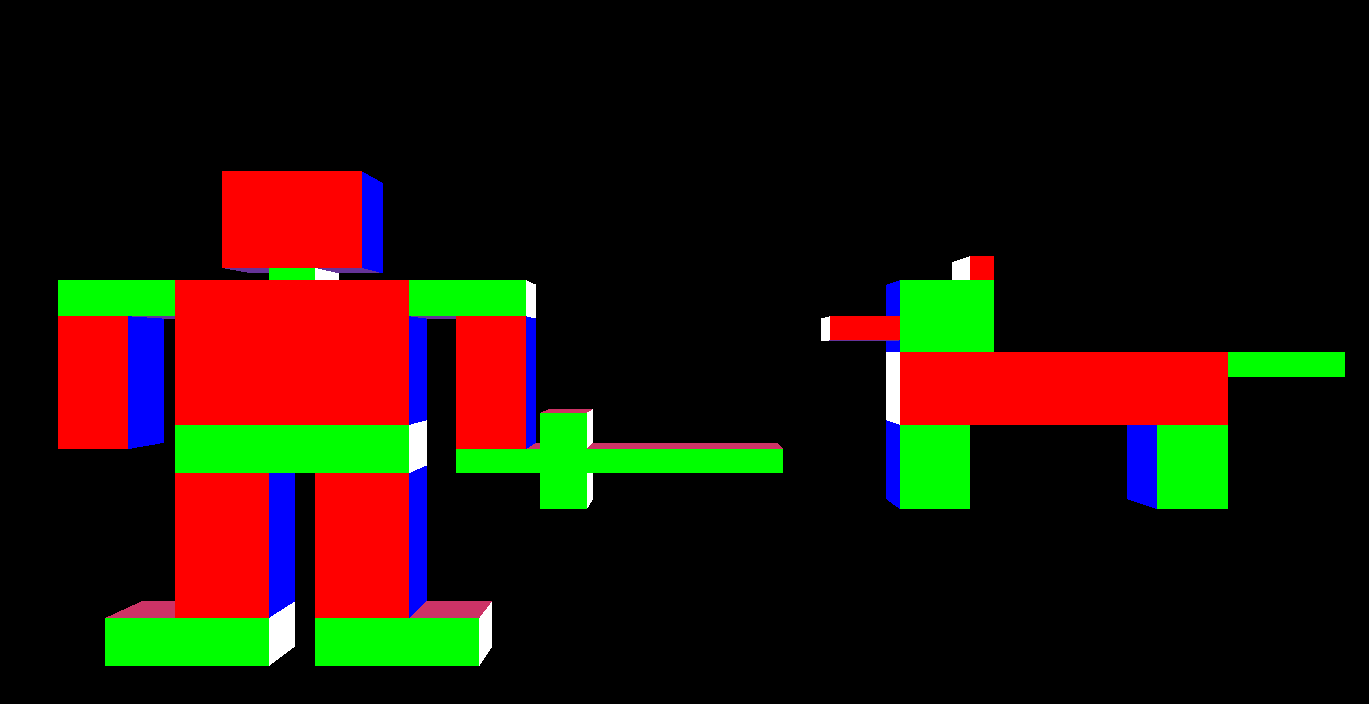
\includegraphics[width=10cm]{images/Transformaciones.png}
\end{center}
\end{figure}
\item \textbf{Ejercicio:} Crear la misma forma de la estrella de la práctica 2 con indices.
\item Deben subir sus ejercicios en Github y colocar la liga en su reporte.
\end{enumerate}
\section{Observaciones y Conclusiones}
\section{Anexos}
\begin{enumerate}
\item Cuestionario previo.
\begin{enumerate}
\item ¿Qué es una clase en c++?
\item ¿Qué es un constructor y destructor de la clase, y cómo se declara en
c++?
\item ¿Cómo se instancia un objeto en c++?
\item Investigar como abrir un archivo en c++.
\item Investigue para qué sirve la función \textbf{glViewport} y que parámetros
recibe.
\item Investigue que es la matriz de Modelo, Vista, Proyección.
\item ¿Qué es una proyección e investigue los tipos de proyecciones, en el
ámbito de gráficos?
\item Que utilidad tiene las funciones \textbf{glm::ortho}, \textbf{glm::frustum} y
\textbf{glm::perspective}, y que son los parámetros que reciben.
\item Para qué sirve la función \textbf{glfwSetWindowPos} y que parámetros recibe.
\item ¿Cuáles son las transformaciones geométricas básicas en tres
dimensiones y sus matrices asociadas?
\item Investigué para sirve la función \textbf{glm::scale}, \textbf{glm::translate}, \textbf{glm::rotate},
y que parámetros reciben.
\end{enumerate}
\item Actividad de investigación previa.
\begin{enumerate}
\item Realizar un \textbf{git pull origin master} y un \textbf{git pull myRepo master}, antes de comenzar la práctica.
\end{enumerate}
\end{enumerate}

%uoooooooooooooooo tumadreuooooooooooooooooooo UOOOOOOOOOOOOOOOOOOOOOOOOOOOOOOOOOOOOOOOOO
%AL FIN SE TERMINA ESTA PUTA MIERDA!!!!
%USEGREAS OSTOJEOGIRN ojeogiek


\end{document}